\documentclass[english,floatsintext,doc]{apa6}

\usepackage{amssymb,amsmath}
\usepackage{ifxetex,ifluatex}
\usepackage{fixltx2e} % provides \textsubscript
\ifnum 0\ifxetex 1\fi\ifluatex 1\fi=0 % if pdftex
  \usepackage[T1]{fontenc}
  \usepackage[utf8]{inputenc}
\else % if luatex or xelatex
  \ifxetex
    \usepackage{mathspec}
    \usepackage{xltxtra,xunicode}
  \else
    \usepackage{fontspec}
  \fi
  \defaultfontfeatures{Mapping=tex-text,Scale=MatchLowercase}
  \newcommand{\euro}{€}
\fi
% use upquote if available, for straight quotes in verbatim environments
\IfFileExists{upquote.sty}{\usepackage{upquote}}{}
% use microtype if available
\IfFileExists{microtype.sty}{\usepackage{microtype}}{}

% Table formatting
\usepackage{longtable, booktabs}
\usepackage{lscape}
% \usepackage[counterclockwise]{rotating}   % Landscape page setup for large tables
\usepackage{multirow}		% Table styling
\usepackage{tabularx}		% Control Column width
\usepackage[flushleft]{threeparttable}	% Allows for three part tables with a specified notes section
\usepackage{threeparttablex}            % Lets threeparttable work with longtable

% Create new environments so endfloat can handle them
% \newenvironment{ltable}
%   {\begin{landscape}\begin{center}\begin{threeparttable}}
%   {\end{threeparttable}\end{center}\end{landscape}}

\newenvironment{lltable}
  {\begin{landscape}\begin{center}\begin{ThreePartTable}}
  {\end{ThreePartTable}\end{center}\end{landscape}}




% The following enables adjusting longtable caption width to table width
% Solution found at http://golatex.de/longtable-mit-caption-so-breit-wie-die-tabelle-t15767.html
\makeatletter
\newcommand\LastLTentrywidth{1em}
\newlength\longtablewidth
\setlength{\longtablewidth}{1in}
\newcommand\getlongtablewidth{%
 \begingroup
  \ifcsname LT@\roman{LT@tables}\endcsname
  \global\longtablewidth=0pt
  \renewcommand\LT@entry[2]{\global\advance\longtablewidth by ##2\relax\gdef\LastLTentrywidth{##2}}%
  \@nameuse{LT@\roman{LT@tables}}%
  \fi
\endgroup}


  \usepackage{graphicx}
  \makeatletter
  \def\maxwidth{\ifdim\Gin@nat@width>\linewidth\linewidth\else\Gin@nat@width\fi}
  \def\maxheight{\ifdim\Gin@nat@height>\textheight\textheight\else\Gin@nat@height\fi}
  \makeatother
  % Scale images if necessary, so that they will not overflow the page
  % margins by default, and it is still possible to overwrite the defaults
  % using explicit options in \includegraphics[width, height, ...]{}
  \setkeys{Gin}{width=\maxwidth,height=\maxheight,keepaspectratio}
\ifxetex
  \usepackage[setpagesize=false, % page size defined by xetex
              unicode=false, % unicode breaks when used with xetex
              xetex]{hyperref}
\else
  \usepackage[unicode=true]{hyperref}
\fi
\hypersetup{breaklinks=true,
            pdfauthor={},
            pdftitle={Supplemental Materials for ``A shifted Wald decomposition of the numerical size-congruity effect: Support for a late-interaction account''},
            colorlinks=true,
            citecolor=blue,
            urlcolor=blue,
            linkcolor=black,
            pdfborder={0 0 0}}
\urlstyle{same}  % don't use monospace font for urls

\setlength{\parindent}{0pt}
%\setlength{\parskip}{0pt plus 0pt minus 0pt}

\setlength{\emergencystretch}{3em}  % prevent overfull lines

\ifxetex
  \usepackage{polyglossia}
  \setmainlanguage{}
\else
  \usepackage[english]{babel}
\fi

% Manuscript styling
\captionsetup{font=singlespacing,justification=justified}
\usepackage{csquotes}
\usepackage{upgreek}



\usepackage{tikz} % Variable definition to generate author note

% fix for \tightlist problem in pandoc 1.14
\providecommand{\tightlist}{%
  \setlength{\itemsep}{0pt}\setlength{\parskip}{0pt}}

% Essential manuscript parts
  \title{Supplemental Materials for ``A shifted Wald decomposition of the
numerical size-congruity effect: Support for a late-interaction
account''}

  \shorttitle{Supplementary material}


  \author{Thomas J. Faulkenberry}

  \def\affdep{{""}}%
  \def\affcity{{""}}%

  \affiliation{
    \vspace{0.5cm}
          \textsuperscript{} Tarleton State University  }

 % If no author_note is defined give only author information if available
      \newcounter{author}
                              \authornote{
            Correspondence concerning this article should be addressed to Thomas J. Faulkenberry, Department of Psychological Sciences, Box T-0820, Tarleton State
University, Stephenville, TX 76401. E-mail: \href{mailto:faulkenberry@tarleton.edu}{\nolinkurl{faulkenberry@tarleton.edu}}
          }
                    

  



  \usepackage{bm}

\usepackage{amsthm}
\newtheorem{theorem}{Theorem}
\newtheorem{lemma}{Lemma}
\theoremstyle{definition}
\newtheorem{definition}{Definition}
\newtheorem{corollary}{Corollary}
\newtheorem{proposition}{Proposition}
\theoremstyle{definition}
\newtheorem{example}{Example}
\theoremstyle{definition}
\newtheorem{exercise}{Exercise}
\theoremstyle{remark}
\newtheorem*{remark}{Remark}
\newtheorem*{solution}{Solution}
\begin{document}

\maketitle

\setcounter{secnumdepth}{0}



In these supplemental materials, I present details on the Bayesian
hypothesis tests performed in the main paper, providing specific
definitions and relevant R code. Then for each test, I provide two
supplements: (1) a plot of the prior and posterior for effect size
\(\delta\), giving a visual representation of the Bayes factor
computation; and (2) a robustness check, showing the effect of prior
choice on the resulting Bayes factor.

\section{Definitions and R-code}\label{definitions-and-r-code}

The Bayesian t-tests described in this paper were performed using the
\texttt{ttestBF} function from the \texttt{BayesFactor} package in R
(Morey \& Rouder, 2012). The \texttt{ttestBF} function implements the
\emph{JZS Bayes factor} computation for t-tests originally described in
Rouder et al. (2009). Recall that the Bayes factor \(B_{01}\) represents
the factor by which the prior odds for hypothesis \(\mathcal{H}_0\) over
hypothesis \(\mathcal{H}_1\) are updated after observing data \(D\).
That is,

\[
\frac{p(\mathcal{H}_0\mid D)}{p(\mathcal{H}_1\mid D)} = B_{01} \times \frac{p(\mathcal{H}_0)}{p(\mathcal{H}_1)}.
\]

\noindent
Computationally, Bayes Theorem implies that \(B_{01}\) is equal to the
ratio of \emph{marginal likelihoods} \(M_0/M_1\), where

\[
M_i = \int_{\bm{\theta}\in \Theta_i} f_i(\bm{\theta}\mid D)\pi_i(\bm{\theta})d\bm{\theta},
\]

\noindent
where \(i=0,1\), \(\Theta_i\) represents the space of parameters
\(\bm{\theta}\) under hypothesis \(\mathcal{H}_i\), \(f_i\) denotes the
likelihood function hypothesis \(\mathcal{H}_i\), given parameters
\(\bm{\theta}\) and data \(D\), and \(\pi_i\) represents the prior
distribution of parameters \(\bm{\theta}\) under hypothesis
\(\mathcal{H}_i\). In the case of a single-sample t-test, the likelihood
\(f_i\) is simply the familiar normal density with parameters \(\mu\)
and \(\sigma\). However, the Bayesian analyst still must choose priors
\(\pi_i\) for each of these parameters.

Rouder et al. (2009) showed that the computation of the marginal
likelihoods \(M_i\) (and, by implication, the Bayes factor \(B_{01}\))
becomes relatively straightforward with a few simple assumptions. First,
instead of placing priors on the mean \(\mu\), we can instead place
priors on the \emph{effect size} \(\delta = \mu/\sigma\). One benefit of
doing so is that the null hypothesis \(\mathcal{H}_0\) may be defined as
\(\delta=0\). Then, Rouder et al. (2009) recommending placing a Cauchy
prior on \(\delta\) (following Jeffreys, 1961) and an inverse-chi-square
prior \(\sigma_{\delta}^2\) (following Zellner and Siow, 1980). As a
result, the formula derived by Rouder et al. (2009) is referred to as
the JZS Bayes factor (named so for Jeffreys, Zellner, and Siow).

The JZS Bayes factor provides the user with a simple default Bayesian
t-test. However, the Bayes factor is sensitive to the choice of prior,
one should take care to be explicit with this choice. With the
\texttt{ttestBF} function, one may easily choose between three default
priors, parameterized as the scale (or width) \(r\) of the Cauchy prior
on effect size \(\delta\). In this context, setting the prior scale to
\(r\) means 50\% of the effect sizes would be expected to be between
\(-r\) and \(+r\). The user may specify this scale via an
\texttt{rscale} argument in the function. Three convenient pre-defined
scales are:

\begin{itemize}
\tightlist
\item
  \enquote{medium}, corresponding to \(r=\sqrt{2}/2\).
\item
  \enquote{wide}, corresponding to \(r=1\)
\item
  \enquote{ultrawide}, corresponding to \(r=\sqrt{2}\)
\end{itemize}

By default, the \texttt{ttestBF} function uses the \enquote{medium}
prior, which is equivalent to starting with a prior belief that effect
sizes are distributed as a Cauchy distribution with scale
\(r=\sqrt{2}/2 \approx 0.707\). However, the choice of prior is
subjective, so it is imperative that a complete Bayesian analysis should
also include an analysis of the sensitivity of the analysis to prior
choice.

In the following sections, I present the details of each Bayesian t-test
that was performed in the original paper. Specifically, I define the
appropriate null and alternative hypotheses, followed by a sensitivity
analyses that shows how the obtained JZS Bayes factor depends on Cauchy
prior scale \(r\).

\section{Bayes factor for median RT}\label{bayes-factor-for-median-rt}

\begin{figure}
\centering
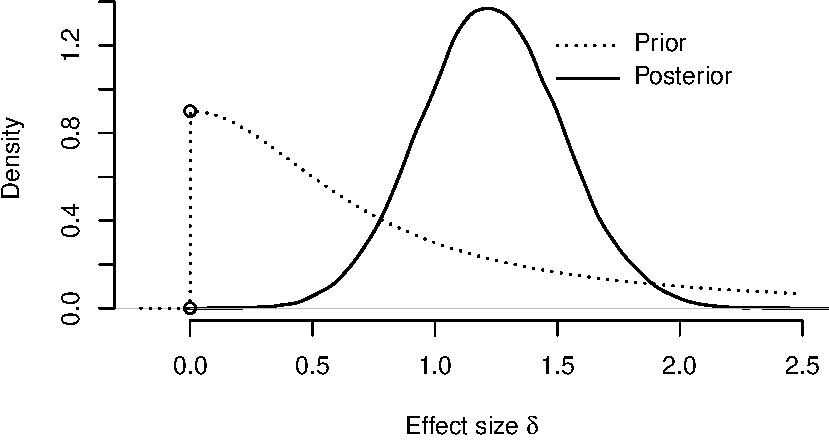
\includegraphics{supplement_files/figure-latex/medianPosterior-1.pdf}
\caption{\label{fig:medianPosterior}Prior and posterior for effect size.
Points on the plot represent the density of the point null in both the
prior and posterior.}
\end{figure}

\begin{figure}
\centering
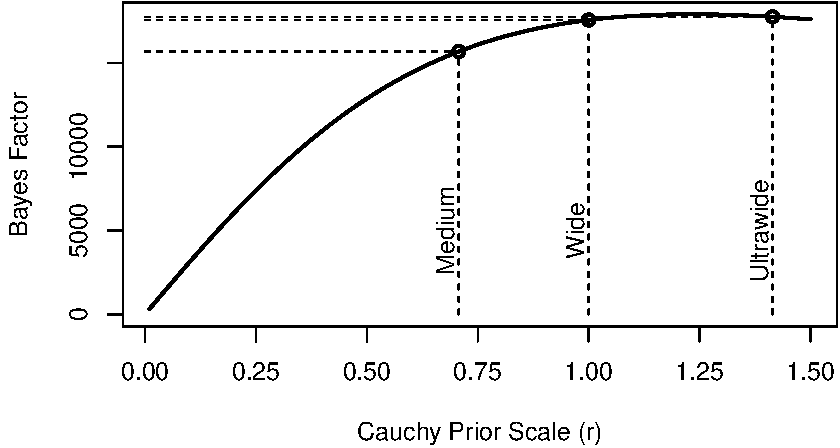
\includegraphics{supplement_files/figure-latex/medianRobustness-1.pdf}
\caption{\label{fig:medianRobustness}Robustness check for Bayes factor in
favor of congruity effect on median RTs.}
\end{figure}

\section{Bayes factor for standard
deviation}\label{bayes-factor-for-standard-deviation}

\begin{figure}
\centering
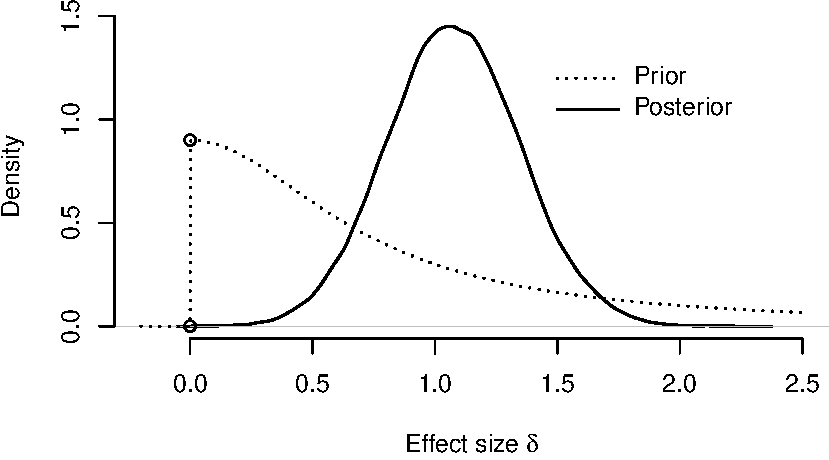
\includegraphics{supplement_files/figure-latex/sdPosterior-1.pdf}
\caption{\label{fig:sdPosterior}Prior and posterior for effect size on
standard deviation. Points on the plot represent the density of the
point null in both the prior and posterior.}
\end{figure}

\begin{figure}
\centering
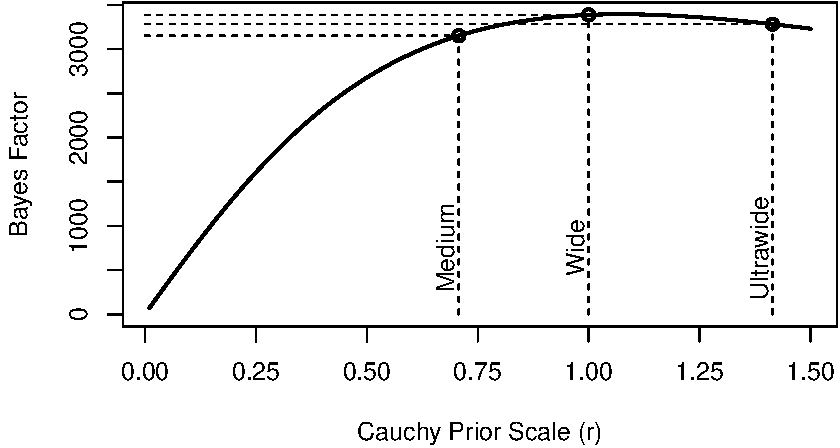
\includegraphics{supplement_files/figure-latex/sdRobustness-1.pdf}
\caption{\label{fig:sdRobustness}Robustness check for Bayes factor in favor
of congruity effect on standard deviations.}
\end{figure}

\section{\texorpdfstring{Bayes factor for drift rate
\(\gamma\)}{Bayes factor for drift rate \textbackslash{}gamma}}\label{bayes-factor-for-drift-rate-gamma}

\begin{figure}
\centering
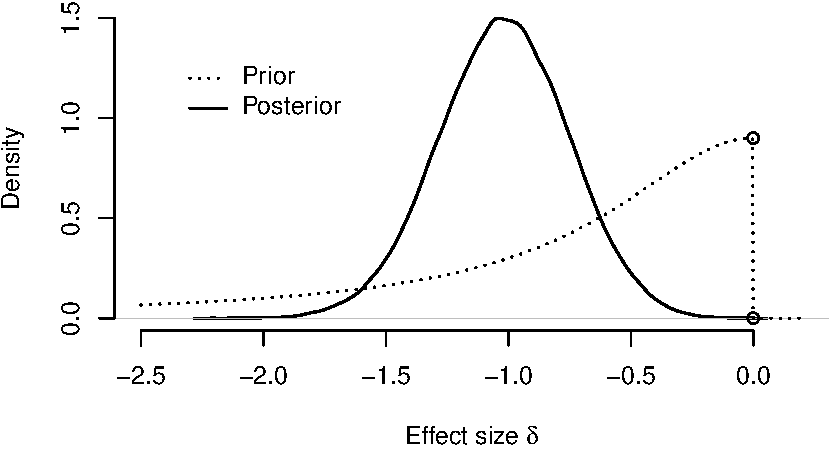
\includegraphics{supplement_files/figure-latex/gammaPosterior-1.pdf}
\caption{\label{fig:gammaPosterior}Prior and posterior for effect size on
drift rate. Points on the plot represent the density of the point null
in both the prior and posterior.}
\end{figure}

\begin{figure}
\centering
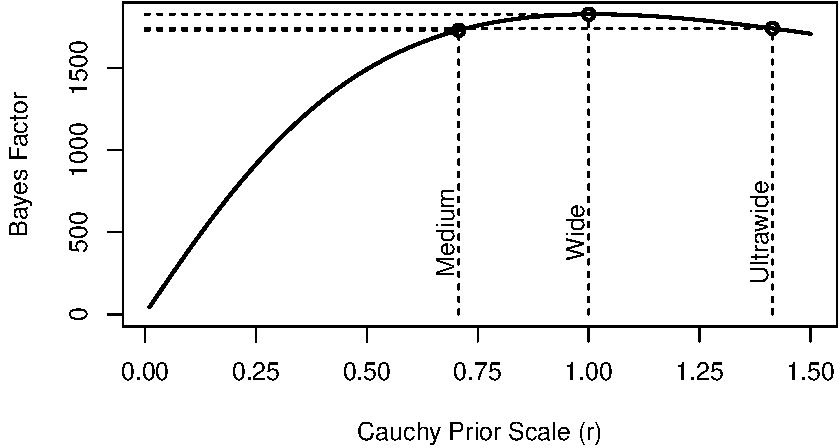
\includegraphics{supplement_files/figure-latex/gammaRobustness-1.pdf}
\caption{\label{fig:gammaRobustness}Robustness check for Bayes factor in
favor of congruity effect on drift rate.}
\end{figure}

\section{\texorpdfstring{Bayes factor for response threshold
\(\alpha\)}{Bayes factor for response threshold \textbackslash{}alpha}}\label{bayes-factor-for-response-threshold-alpha}

\begin{figure}
\centering
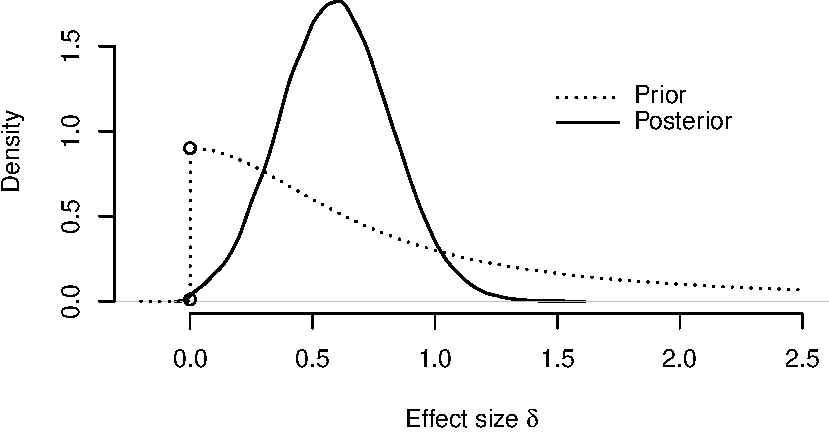
\includegraphics{supplement_files/figure-latex/alphaPosterior-1.pdf}
\caption{\label{fig:alphaPosterior}Prior and posterior for effect size on
response threshold. Points on the plot represent the density of the
point null in both the prior and posterior.}
\end{figure}

\begin{figure}
\centering
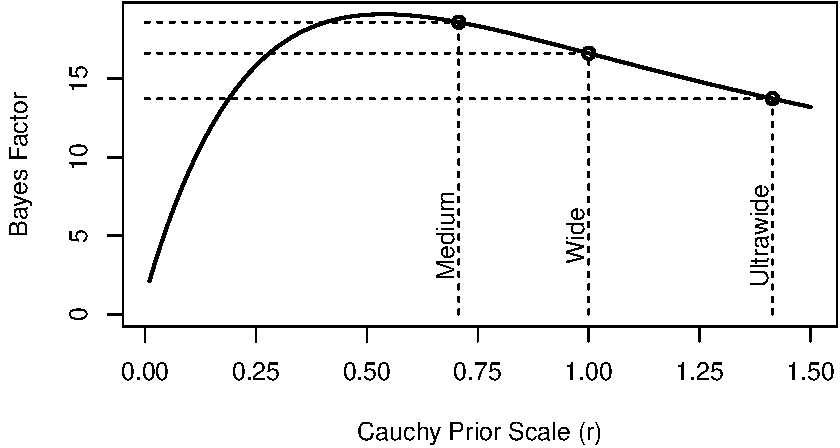
\includegraphics{supplement_files/figure-latex/alphaRobustness-1.pdf}
\caption{\label{fig:alphaRobustness}Robustness check for Bayes factor in
favor of congruity effect on response threshold.}
\end{figure}

\section{\texorpdfstring{Bayes factor for nondecision time
\(\theta\)}{Bayes factor for nondecision time \textbackslash{}theta}}\label{bayes-factor-for-nondecision-time-theta}

\begin{figure}
\centering
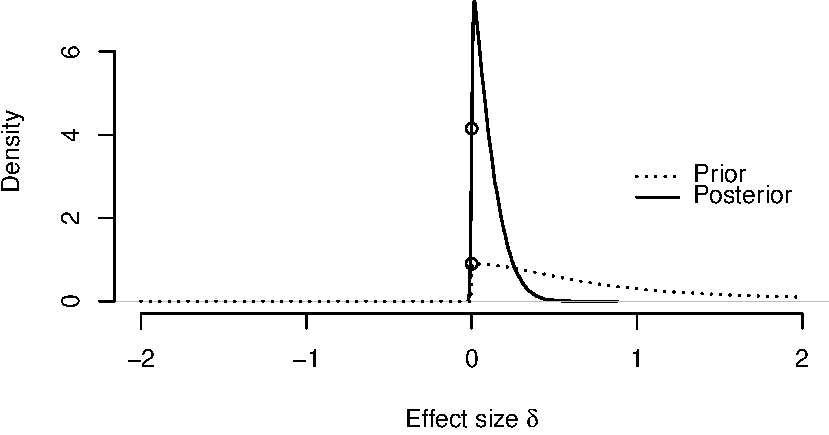
\includegraphics{supplement_files/figure-latex/thetaPosterior-1.pdf}
\caption{\label{fig:thetaPosterior}Prior and posterior for effect size on
nondecision time. Points on the plot represent the density of the point
null in both the prior and posterior.}
\end{figure}

\begin{figure}
\centering
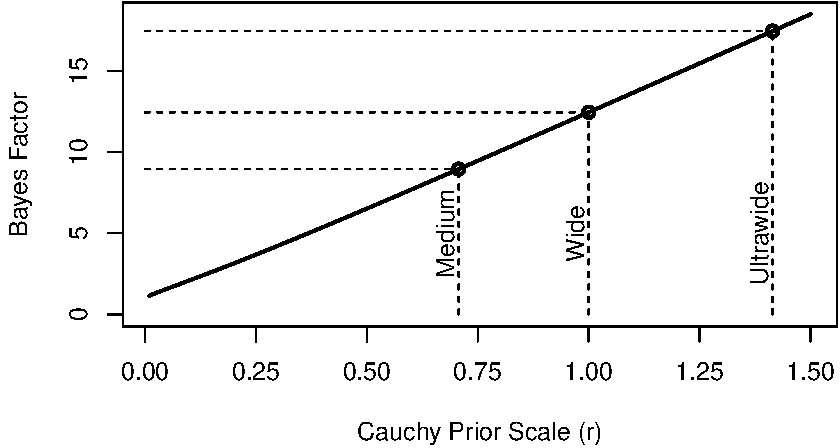
\includegraphics{supplement_files/figure-latex/thetaRobustness-1.pdf}
\caption{\label{fig:thetaRobustness}Robustness check for Bayes factor in
favor of null effect of congruity effect on nondecision time}
\end{figure}

TODO - fix point null positions in posterior densities. Probably need to
use \texttt{logspline} package

\newpage

\section{References}\label{references}

\setlength{\parindent}{-0.5in} \setlength{\leftskip}{0.5in}






\end{document}
